\subsection{Ribbon-10L parametric equation}
\begin{table}[ht]
	\begin{center}
		\begin{tabular}[top]{ |p{16.0 cm}| }
			\rowcolor{LIGHTCYAN}			
			%% \hline \multicolumn{1}{|c|}{\textbf{Part 5/5 Circle and AstEpi parametric curves}} \\ [1.0ex]
			
	%%	double t = 4.0*(u - 0.50); // TRANSORMATION EQUATION
	%%	double scaleup = 1.0;
	%%	double x = (t*t);
	%%	return (scaleup)*(x);	
			
	%%	double t = 4.0*(u - 0.50); // TRANSORMATION EQUATION
	%% 	double scaleup = 1.0;
	%%	double y = (t*t*t) - 3*(t) + 3;
	%%	return (scaleup)*(y);
			
			
			\hline  \textbf{No. 9 - Ribbon-10L parametric curve}\\
			\begin{eqnarray}
				t(u) & = & 4(u - 0.50) \nonumber \\
				x(u) & = & t^2 \nonumber \\   
				y(u) & = & t^3 - 3t + 3 \nonumber \\
				u & \in & [0.0, 1.0] \nonumber
			\end{eqnarray}
			
			Open ended curve\\
			Overall Single loop, smooth convex curves\\
			Reflection x-axis: non-symmetrical\\
			Reflection y-axis: non-symmetrical\\
			\frame{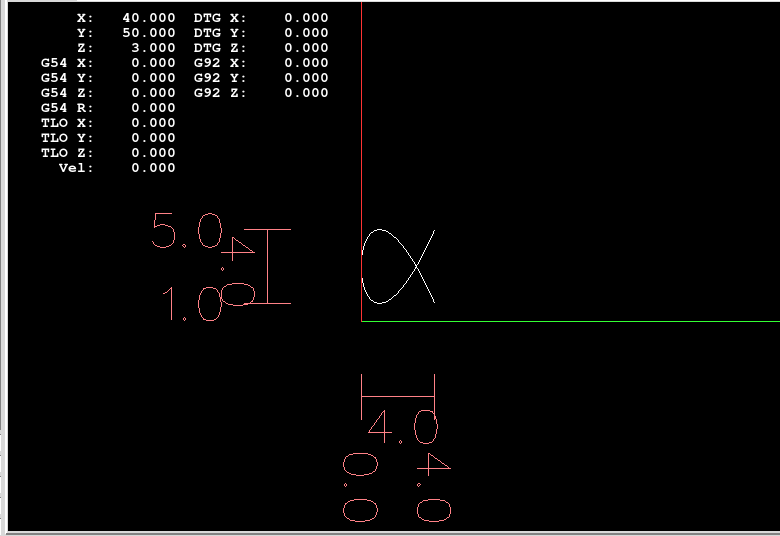
\includegraphics[width=0.560\textwidth]{./07-images/img-Ch5/RIBBON-10L-Axis.png}}
			\frame{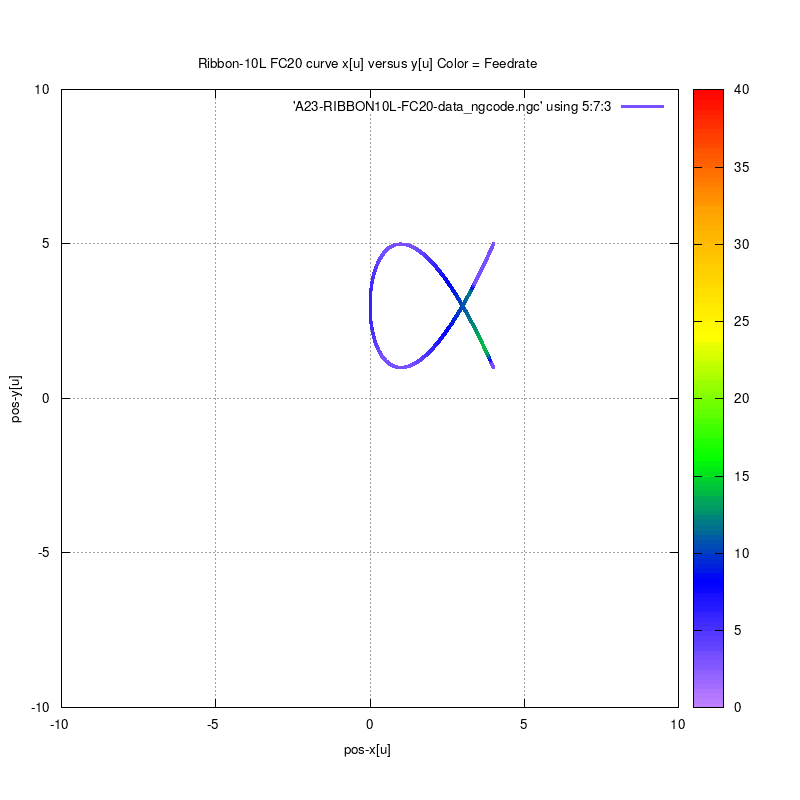
\includegraphics[width=0.394\textwidth]{./07-images/img-Ch5/RIBBON-10L-Feedrate.png}}\\
			
			\hline
		\end{tabular}
		\caption{Ribbon-10L equations and dimensions}		
		\label{table:Ribbon-10L equations and dimensions}
	\end{center}
\end{table}  
